\chapter*{Introduction \& problem definition}
This is the report of Paolo Ginefra's solution to the "Image Analysis and Computer Vision" homework 2024/25.
All the referenced code is available in the GitHub Repository.

\section{Problem definition}
In this section, the problem at hand will be described in detail referencing the "Homework Assignment 2024-25" document.
\subsection{Scene description}
 A piece of furniture is a rectangular parallelepiped, whose width (along the X-axis) is $l = 1$. 
The other dimensions, namely the depth $m$ along the $Y$ axis and the height $h$ along the $Z$-axis are 
unknown. In addition, a horizontal circumference (i.e., parallel to the X-Y plane) is visible. 
Furthermore, an unknown horizontal planar curve is also visible, placed at midheight $h$/2. 

\begin{figure}[!ht]
\centering
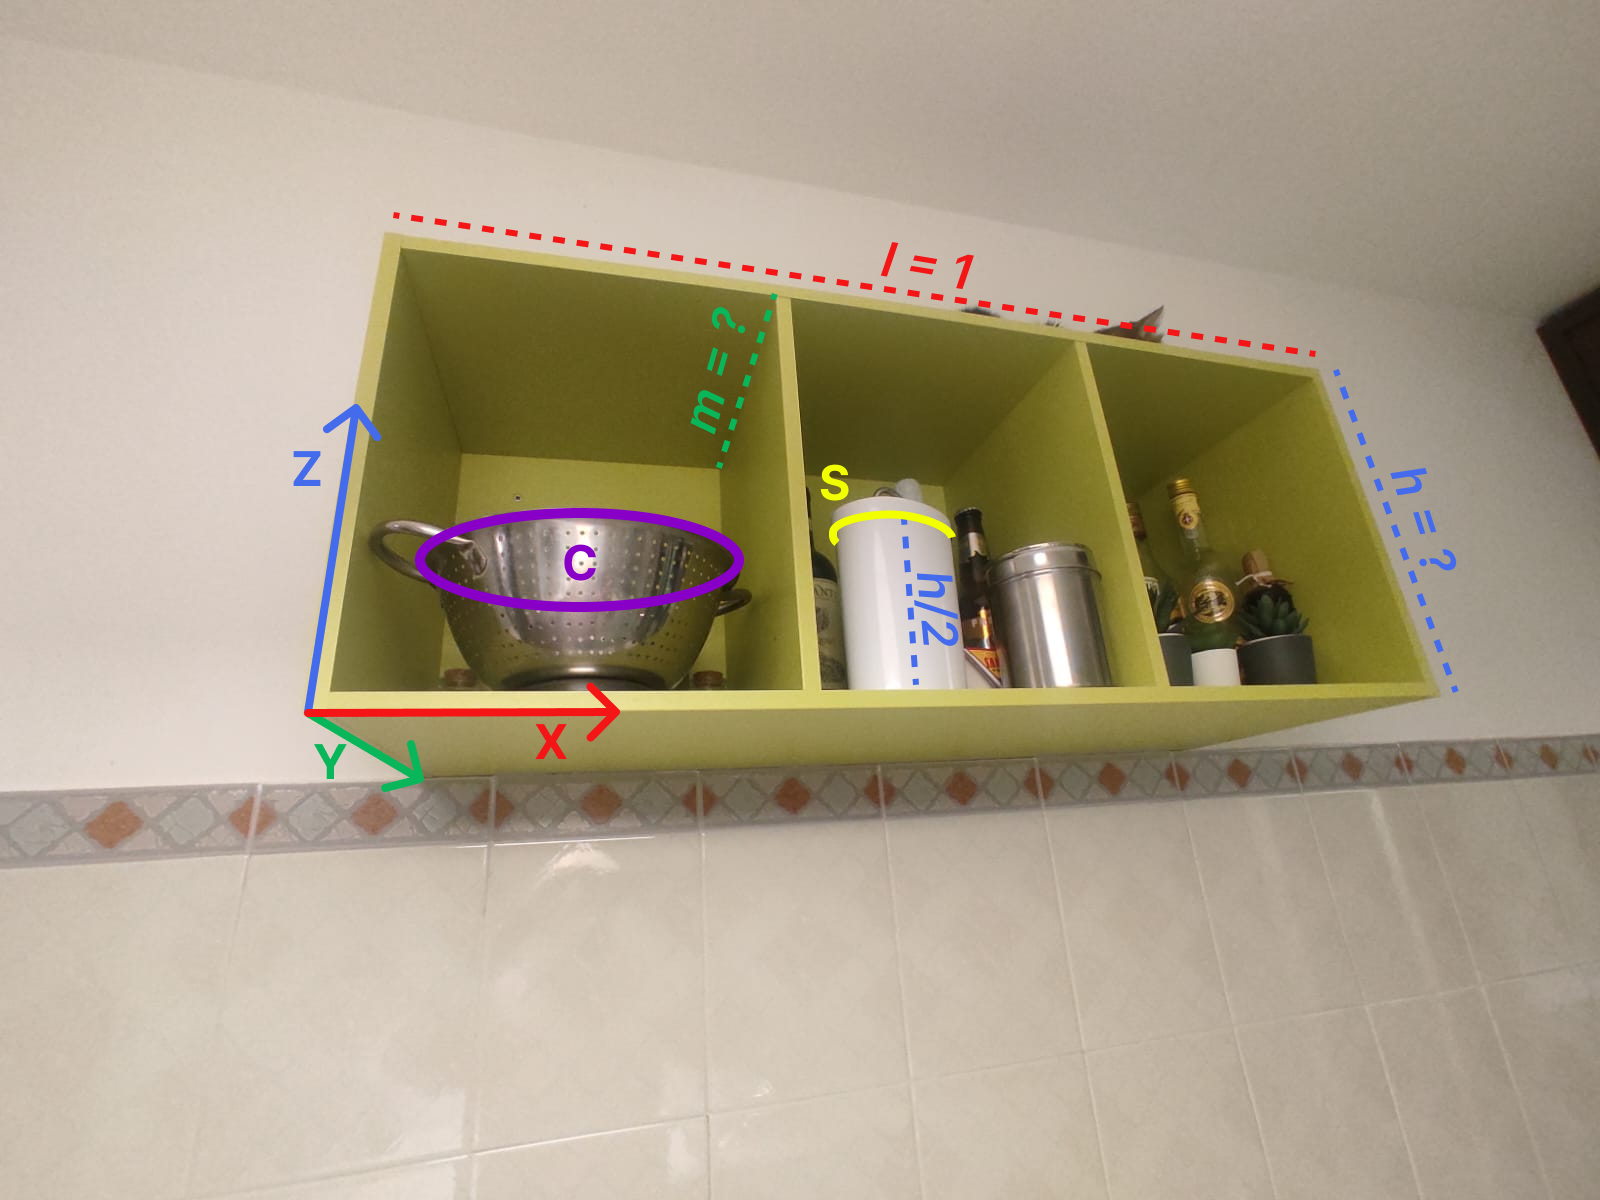
\includegraphics[height=9.5cm, width=\textwidth, keepaspectratio]{Report/Images/Introduction/Scene Description.png}
\caption{\label{fig:SceneDescription}The Scene Description}
\end{figure}

\subsection{Image Description}
A single image is taken of the above rectangular parallelepiped by an uncalibrated, zero
skew, camera. (Its calibration matrix $K$ depends on four unknown parameters, namely $f_x$, $f_y$ and 
the two pixel coordinates $U_O$, $V_O$ of the principal point). A set of lines parallel to X-axis are visible, and their images $l_1$, $l_2$ and $l_3$ are extracted; a set of lines parallel to the $Y$-axis are visible and their images  $m_1$, $m_2$, $m_3$, $m_4$, $m_5$ and $m_6$ are extracted; a set of vertical lines (i.e., parallel to the $Z$
axis) are also visible and their images $h_1$, $h_2$, $h_3$ and $h_4$ are extracted.  In addition, both the image $C$ of the circumference and the image $S$ of the unknown horizontal curve are also extracted.  

\begin{figure}[!ht]
\centering
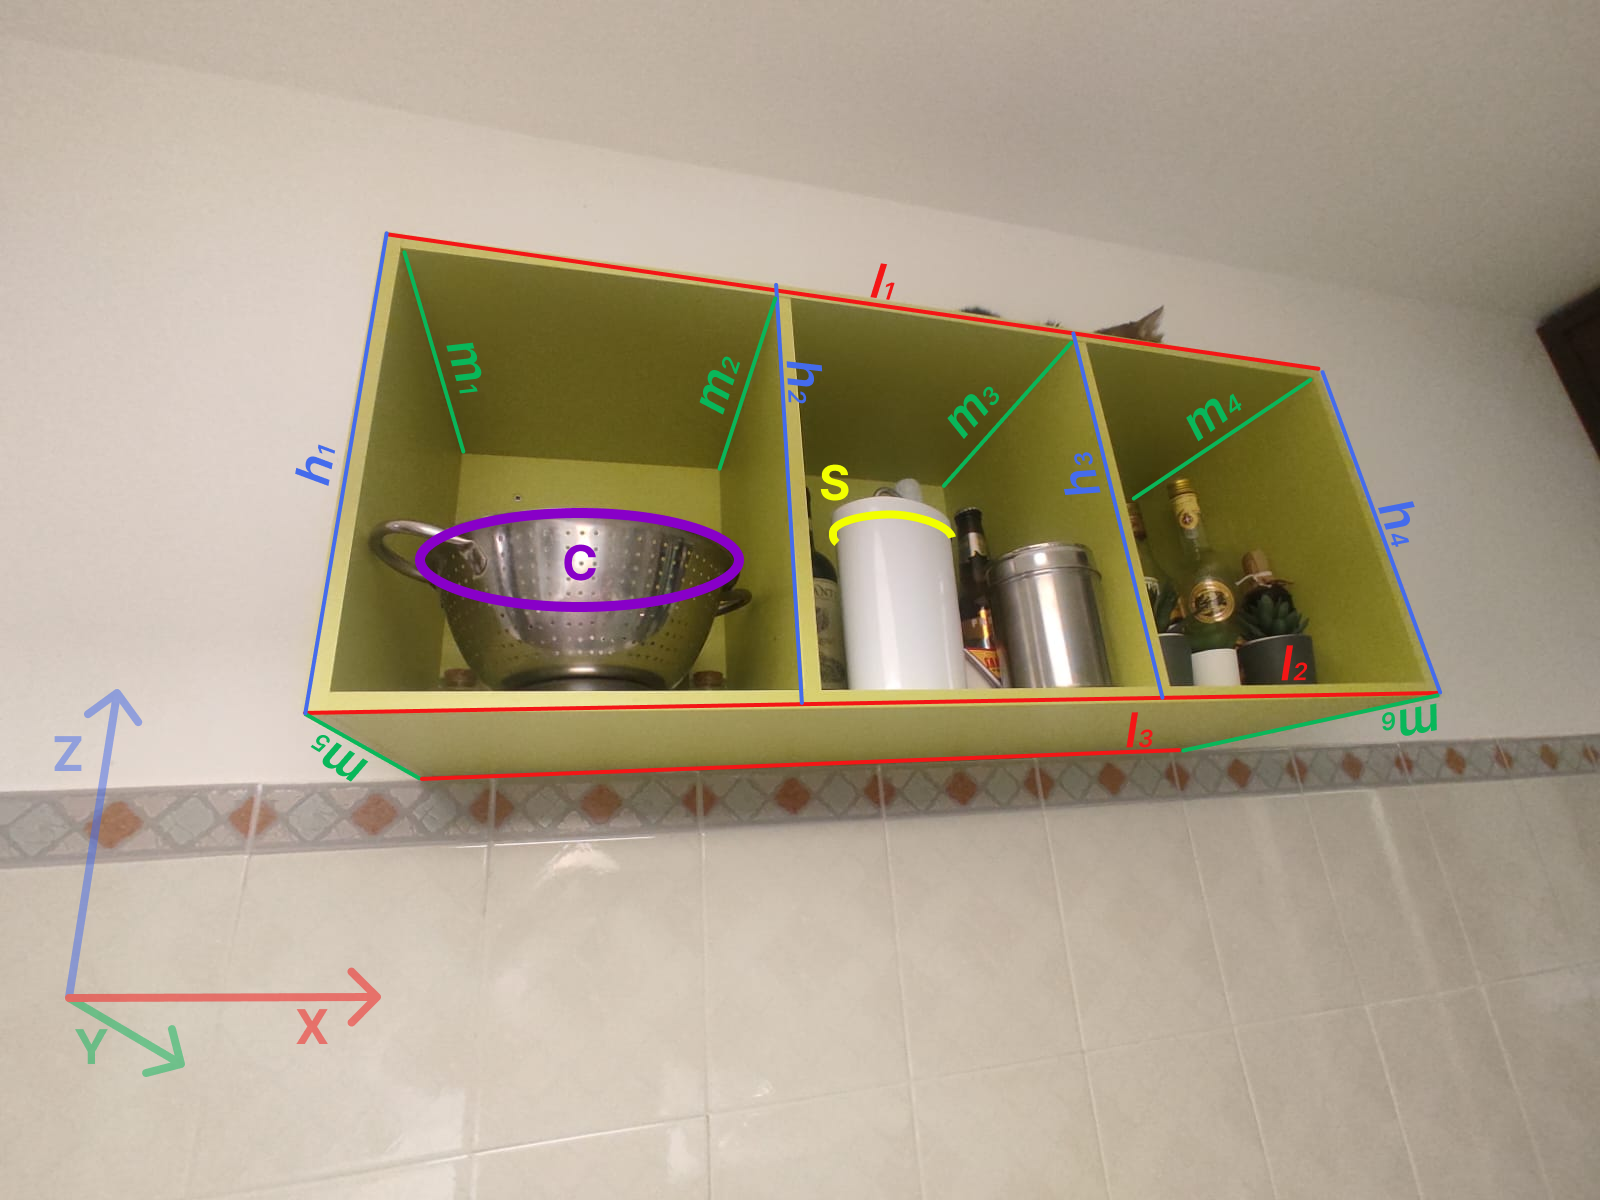
\includegraphics[height=9.5cm, width=\textwidth, keepaspectratio]{Report/Images/Introduction/Image Description.png}
\caption{\label{fig:SceneDescription}The Scene Description}
\end{figure}

\subsection{Part1 - Theory}
\begin{enumerate}
    \item From the $l_i$ and $m_i$ lines, find the vanishing line $l'_\infty$ of the horizontal plane. 
    \item Using the results of the previous point, find a (Euclidean) rectification mapping $H_R$ for a horizontal plane (e.g., the lower horizontal face of the parallelepiped), and compute the depth $m$ of the parallelepiped.  
    \item From the results of the previous points, use the lines $h_i$ to find the calibration matrix $K$. 
    \item Using the results of the previous points, determine the height $h$ of the parallelepiped.  
    \item Using $S$ and the results of previous points, compute the X-Y coordinates of a dozen points (at your choice) of the unknown horizontal curve. 
    \item Using $K$, localize the camera with respect to the parallelepiped.
\end{enumerate}

\subsection{Part2 - Matlab}
\begin{enumerate}
    \item Consider the image "Look-outCat.png". Using feature extraction techniques (including those already implemented in Matlab) plus possible manual intervention, extract the images of useful lines and both the image $C$, of the circumference and the image $S$ of the other planar curve. 
    \item Write a Matlab program that implements the solutions to problems 1 – 6 and show the obtained results. 
    \item Plot the rectified curve $S$ and show different views of the recovered 3D model of the 
rectangular parallelepiped. 
\end{enumerate}

\section{Document structure}
Since the Theory and the Matlab code have a significant overlap, they are presented in parallel following the numbering of the Matlab part. The $n-th $ Theory task takes the numbering $2.n$. For each part, the actual code is not reported since it is easily accessible and documented in the GitHub Repository.